% 9 variables in here:
% h_1 = 10.0, h_2 = 10.0, h_3 = 10.0, ux_1 = 0.0, ux_2 = 0.0, ux_3 = 0.0, uy_1 = 0.0, uy_2 = 0.0, uy_3 = 0.0
\begin{figure}[h]
\centering
  \subfigure[1st basis function, $x$-momentum -- 1st basis function $y$-momentum -- 2nd basis function, $y$-momentum -- 3rd basis function, $y$-momentum] {
    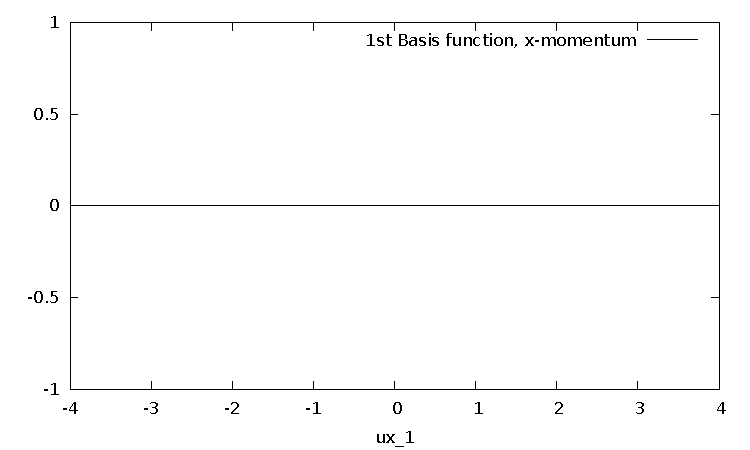
\includegraphics[scale=\zoomfactor]{{{standardwerte_nach_ux_ord1/10.0_10.0_10.0_y_0.0_0.0_0.0_0.0_0.0f00}}}
  }
  % \subfigure[] {
  %   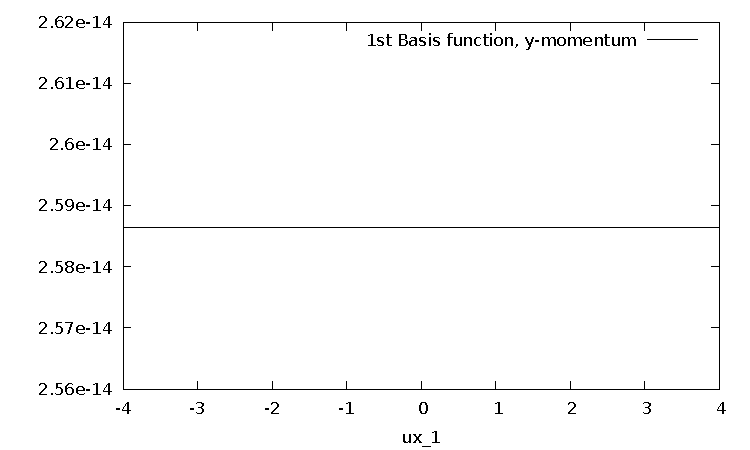
\includegraphics[scale=\zoomfactor]{{{standardwerte_nach_ux_ord1/10.0_10.0_10.0_y_0.0_0.0_0.0_0.0_0.0f01}}}
  % }
  \subfigure[2nd basis function, $x$-momentum -- 3rd basis function, $y$-momentum] {
    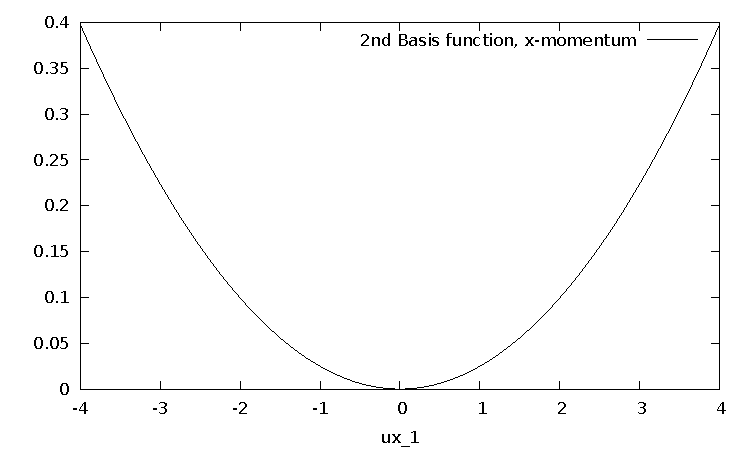
\includegraphics[scale=\zoomfactor]{{{standardwerte_nach_ux_ord1/10.0_10.0_10.0_y_0.0_0.0_0.0_0.0_0.0f02}}}
  }
  % \subfigure[] {
  %   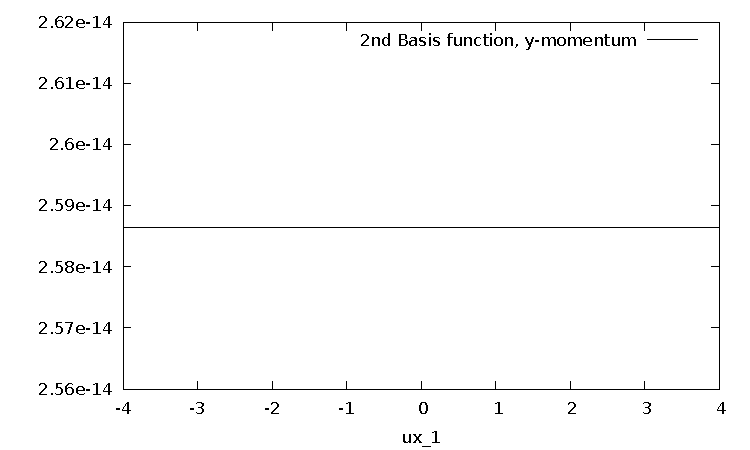
\includegraphics[scale=\zoomfactor]{{{standardwerte_nach_ux_ord1/10.0_10.0_10.0_y_0.0_0.0_0.0_0.0_0.0f03}}}
  % }
  % \subfigure[] {
  %   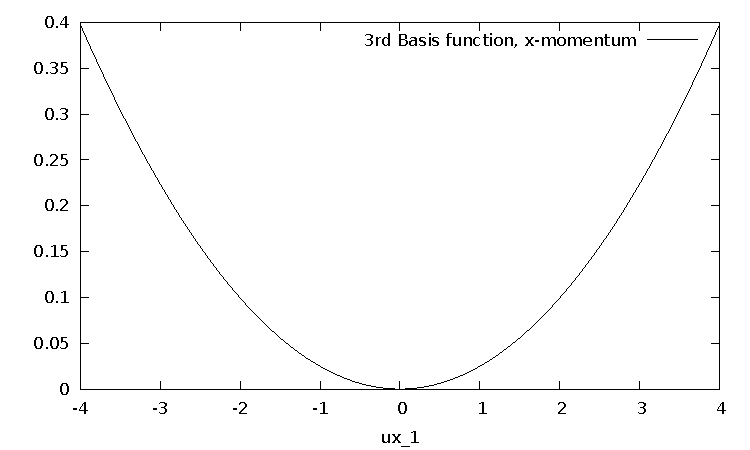
\includegraphics[scale=\zoomfactor]{{{standardwerte_nach_ux_ord1/10.0_10.0_10.0_y_0.0_0.0_0.0_0.0_0.0f04}}}
  % }
  % \subfigure[] {
  %   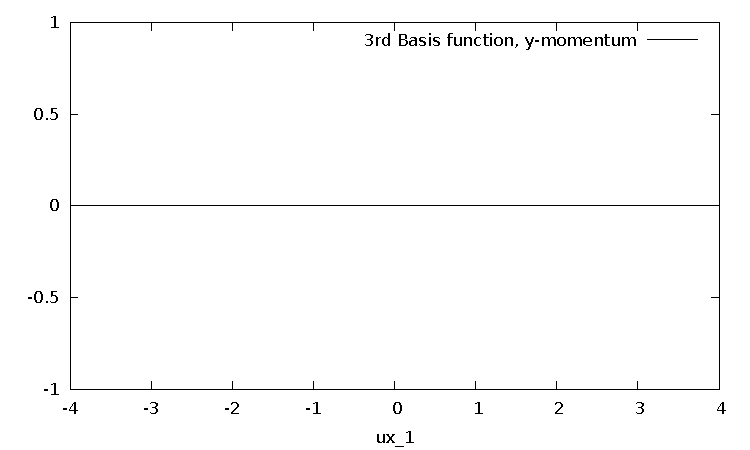
\includegraphics[scale=\zoomfactor]{{{standardwerte_nach_ux_ord1/10.0_10.0_10.0_y_0.0_0.0_0.0_0.0_0.0f05}}}
  % }
\caption{Error plots for order 1. Values of variables are 
  $h_1=10, h_2 = 10 , h_3 = 10,
  u_{x,2} = 0 , u_{x,3} = 0 ,
  u_{y,1}=0, u_{y,2} = 0 , u_{y,3} = 0$. $u_{x,1}$ is varying.}
\label{fig:stiffness-analysis-order-1-standard-values-ux1}
\end{figure}

%%% Local Variables:
%%% TeX-master: "../results.tex"
%%% End:
